\documentclass[14pt]{extreport}
\usepackage{gost}
\usepackage{hyperref}
\usepackage{makecell}
\usepackage{ragged2e}
\justifying

\makeatletter
\@addtoreset{figure}{part}
\makeatother
\renewcommand{\thefigure}{\arabic{figure}}
\renewcommand{\thetable}{\arabic{table}}




\begin{document}
\pagestyle{empty} 

\includepdf[pages=-,pagecommand={}]{titulCourse.pdf}

\pagestyle{plain}
\tableofcontents
 



\intro 

В данном отчете будет приведена основная идея мобильного приложения OptiTune, будут описаны функции, основные пользователи приложения и интерфейс, а также будет проведена оценка рынка и обзор аналогов.


\chapter{ОСНОВНАЯ ИДЕЯ МОБИЛЬНОГО ПРИЛОЖЕНИЯ\label{chapter1}}
\section{Описание основных функций приложения}

Мобильное приложение OptiTune предназначено для использования профессиональными стрелками, охотниками и военными. Оно позволит подобрать тюнинг для гладкоствольного и нарезного оружия, улучшая там самым качество стрельбы.

Используя приложение, пользователи смогут найти конкретное оружие, которое у них уже имеется или которое они только собираются приобрести, а также добавить его в избранное. Пользователи смогут посмотреть весь доступный тюнинг на их оружие и увидеть, как он будет выглядеть отдельно и на оружии, благодаря использованию 3D-модели. Эту модель можно будет масштабировать и разлядывать с разных ракурсов, что позволит пользователю оценить насколько внешне подходит данная комплектация.

Для каждой запчасти будет доступна к просмотру и сравнению подробная характеристика, в которую входят такие параметры как высота, ширина, толщина, материал, из которого изготовлена данная запчасть, и прочее. По этим параметрам можно настроить сортировку и ускорить поиск. Важным показателем при выборе тюнинга является вес. Поэтому при добавлении той или иной запчасти в комплектацию будет наглядно изменяться показатель веса всего оружия. Более того, будет показана примерная цена запчастей, основанная на анализе рынка. Таким образом, пользователи смогут правильнее оценить эти критерии и сделать выбор, который подходит именно им, а также добавить его в избранное.

Еще одной функцией приложения являются комментарии пользователей и оценка ими тюнинга. Важно отметить, что функция написания будет доступна только зарегистрированным пользователям. Оценки будут выставляться по определенным критериям, например по критерию удобства использования. Также пользователи смогут прикреплять к своим комментариям картинки и видеозаписи с готовым тюнингом. Все комментарии будут проверяться модератором, чтобы избежать нежелательной информации.

В случае если у пользователя возникнут вопросы по техническим характеристикам или выбору, ему необходимо зарегистрироваться в приложении. Так, он сможет обратиться через специальное окно к онлайн-консультанту, который постарается ответить на все вопросы в ближайшее время.

Итак, подведем итоги по функционалу, который будет представлен в приложении:
\begin{itemize}
\item подбор тюнинга на основе конкретного оружия;
\item просмотр и сравнение характеристик запчастей;
\item добавление в избранное понравившегося тюнинга;
\item написание и просмотр комментариев пользователей;
\item оценивание тюнинга по различным критериям;
\item помощь онлайн-консультанта.
\end{itemize}

\newpage
\section{Основные пользователи приложения}

Основными пользователями приложения являются люди, которые заинтересованы в тюнинге своего оружия. Им будут доступны такие функции как просмотр и подбор тюнинга, а также сравнение и добавление запчастей в закладки. Для зарегистрированных пользователей будет доступно написание комментариев, оценка запчастей и помощь онлайн-консультанта, в то время как для остальных пользователей будет доступен только просмотр оценок и комментариев этих пользователей.

Для того, чтобы не допускать нежелательные комментарии и спам до обычных пользователей, необходим модератор, который будет отслеживать подобные комментарии.

Для помощи в каких-либо вопросах по характеристикам тюнинга и выбору нужен онлайн-консультант, имеющий необходимые знания и отвечающий на эти вопросы.

Также важен менеджер, который будет обновлять информацию в приложении, например добавлять или удалять характеристики тюнинга.

\newpage
\section{Прототип интерфейса будущего приложения}

В данном разделе представлен прототип интерфейса будущего приложения (рисунок \ref{fig1}):

\begin{figure}[H]
\centerline{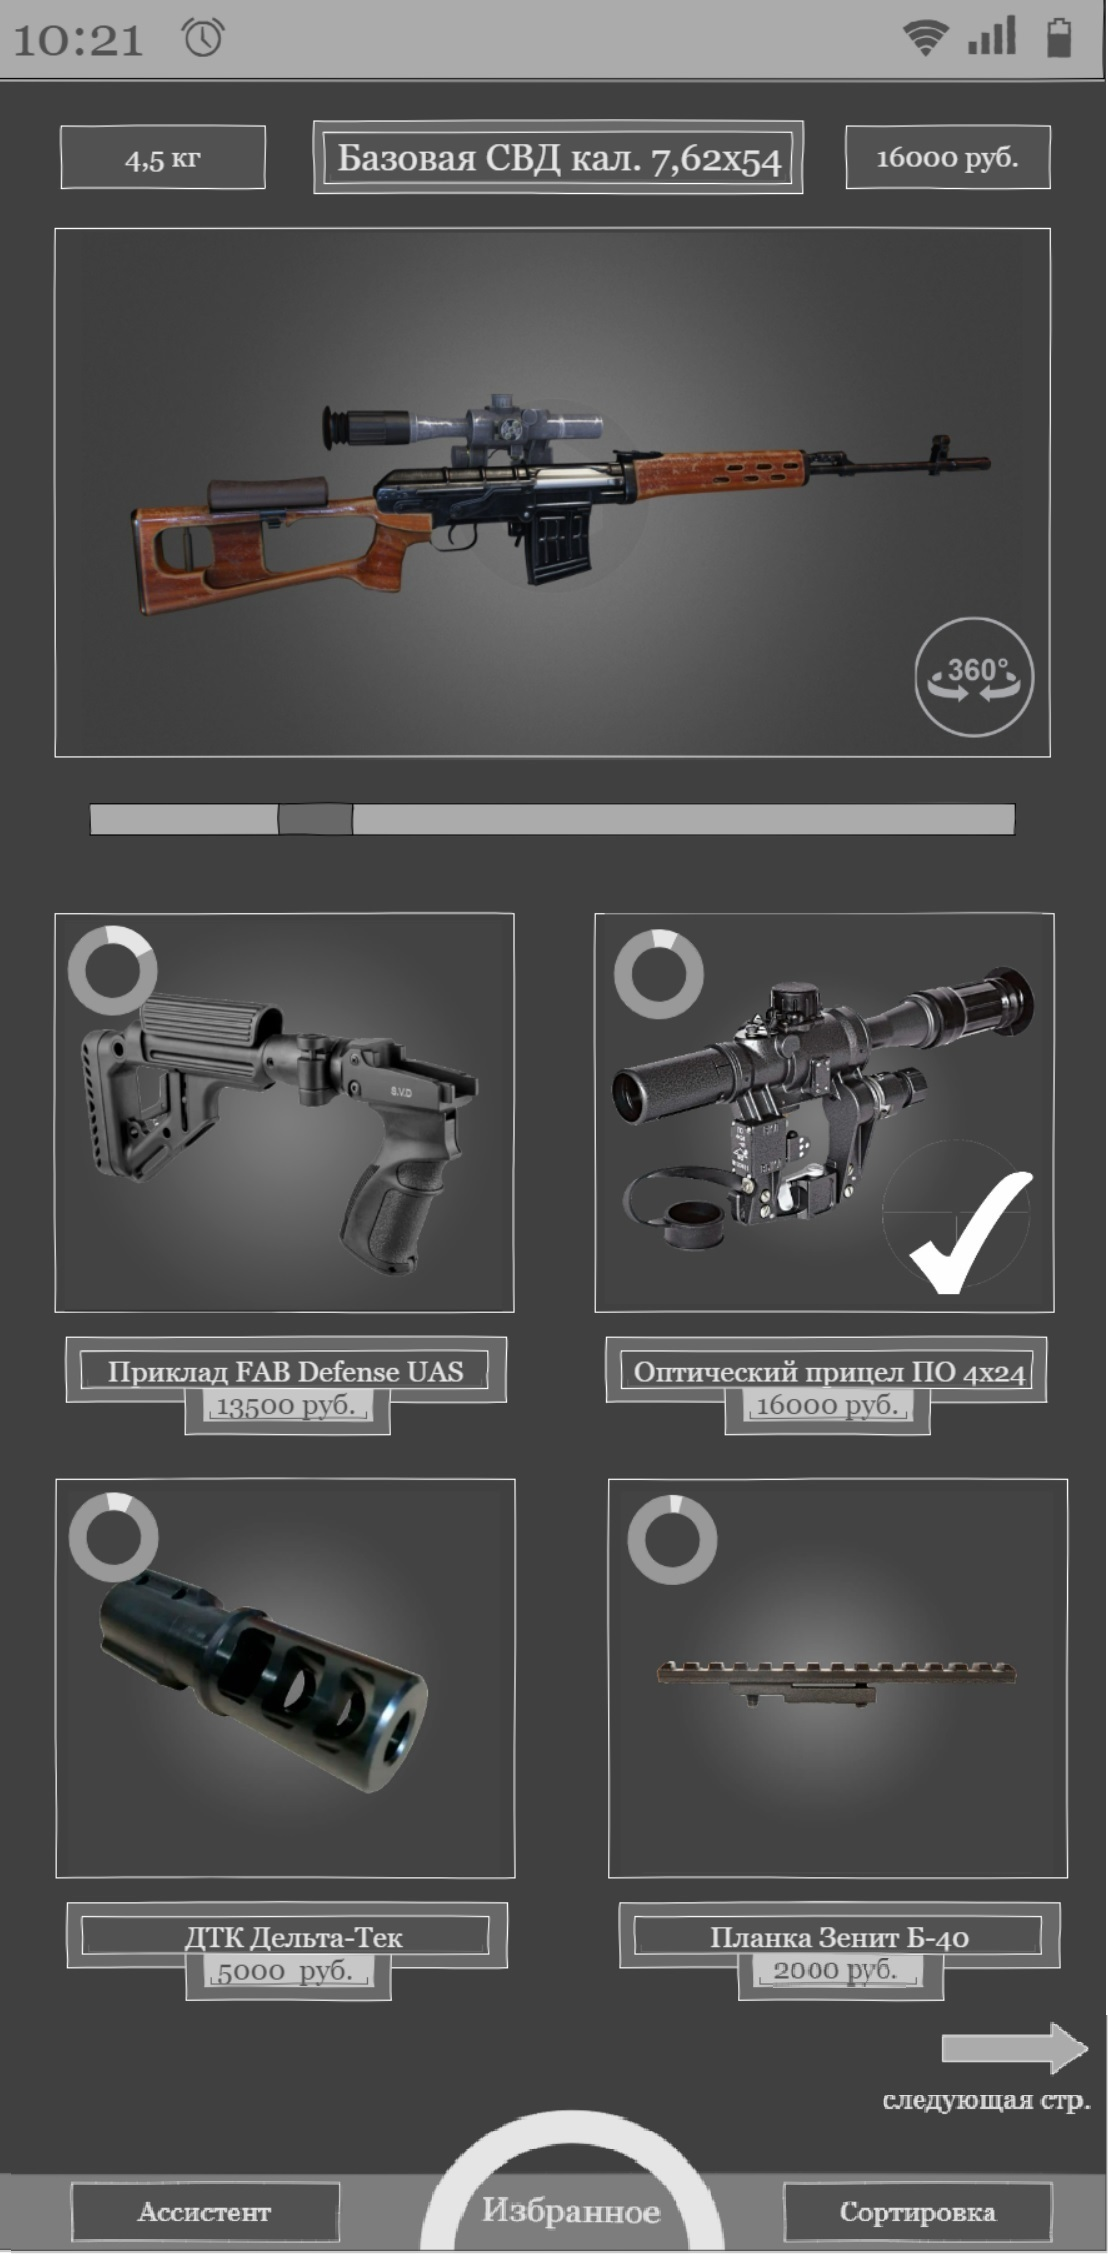
\includegraphics[width=0.55\linewidth]{pic}}
\caption{Прототип интерфейса}
\label{fig1}
\end{figure}


\chapter{ОЦЕНКА РЫНКА\label{chapter2}}
\section{Обзор аналогов, представленных на рынке}

При анализе зарубежного и российского рынка приложений не нашлось аналогов. Лишь среди сайтов можно было отыскать что-то похожее.

Интернет-магазин товаров для тюнинга оружия и аксессуаров Custom Guns \cite{bib1}. На данном сайте можно найти и купить запчасти. На сайте есть иллюстрации к каждой запчасти, цена и подробные характеристики. Так же как и у моего приложения здесь есть система оценивания и онлайн-ассистента. Однако на сайте нельзя сравнивать и добавлять в избраннное запчасти, также нельзя посмотреть как тюнинг будет выглядеть на оружии, зато настроен интернет-магазин.

В двух других интернет-магазинах, QUARTA \cite{bib2} и Guns Parts \cite{bib3}, так же присутствовали иллюстрации к тюнингу, сортировка, отзывы о товаре и онлайн-ассистент. В отличие от первого сайта, здесь пользователь может зайти в личный кабинет и добавить товары в избранное. Однако все еще нельзя посмотреть внешний вид оружия с тюнингом. 

Во всех трех системах пользователи совпадают с пользователями приложения. Важно отметить, что довольно сложно сделать 3D-модели для всех запчастей, поэтому большая часть систем не воплощает эту идею. 


\newpage
\section{Обоснование необходимости разработки приложения}

Проанализировав рынок приложений, не сложно заметить, что конкуренции в этой области нет, а также это уникальное приложение, которое может заинтересовать профессиональных стрелков. Поэтому, действительно, есть смысл реализовать данное приложение.


\conclusions

Был составлен отчет, в котором приведена идея приложения OptiTune, описаны основные функции и пользователи, а также приведен прототип будущего приложения. Была проведена оценка рынка и обзор аналогов, на основе которых были составлены некоторые выводы.



\newpage
\begin{thebibliography}{99}

\bibitem{bib1} Custom Guns: официальный сайт. – URL: \url{https://custom-guns.ru} (Дата обращения 11.10.2022).

\bibitem{bib2} QUARTA: официальный сайт. – URL: \url{https://quarta-hunt.ru} (Дата обращения 11.10.2022).

\bibitem{bib3} Guns parts: официальный сайт. – URL: \url{https://www.gunsparts.ru} (Дата обращения 11.10.2022).



\end{thebibliography}







\end{document}
